\providecommand{\main}{../main}
\documentclass[../main/main.tex]{subfiles}


\setcounter{section}{0}
\renewcommand{\thesection}{\textbf{\Alph{section}}}
\renewcommand{\thesubsection}{\textbf{\arabic{subsection}}}
    

\begin{document}

\section{Appendix}
\label{sec:appendix}

\subsection{Low-level features distributions}
\label{ssec:appendix_low_features}

% \begin{figure*}[!h]
%     \begin{minipage}[c]{0.333\linewidth}
%         \vspace{0pt}
%         \centering
%         \subfloat[Lepton \( p_{\text{T}} \)]{
%             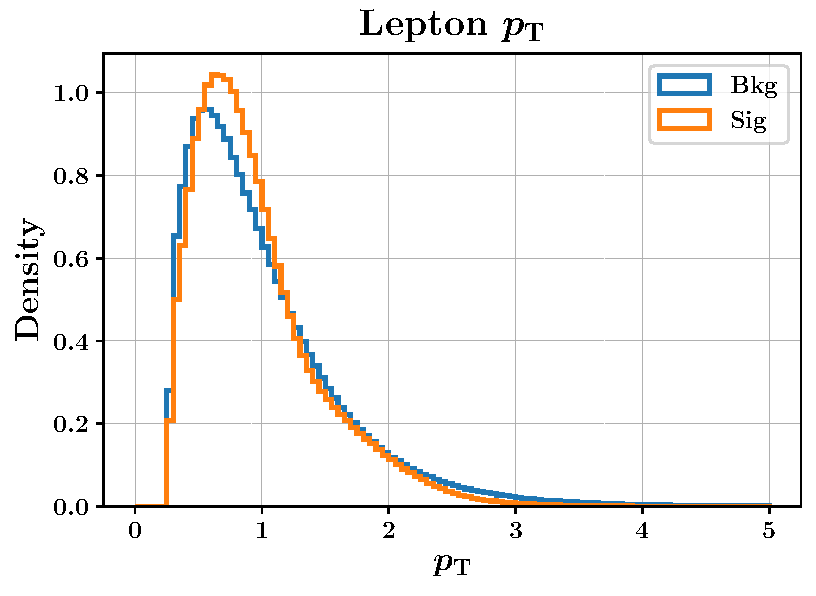
\includegraphics[width=\textwidth]{images/theory/lowlevel/l_pt.pdf}
%             \label{fig:appendix_low_features_leptonic_l_pt}
%         }
%     \end{minipage}%
%     \begin{minipage}[c]{0.333\linewidth}
%         \vspace{0pt}
%         \centering
%         \subfloat[Lepton \( \eta \)]{
%             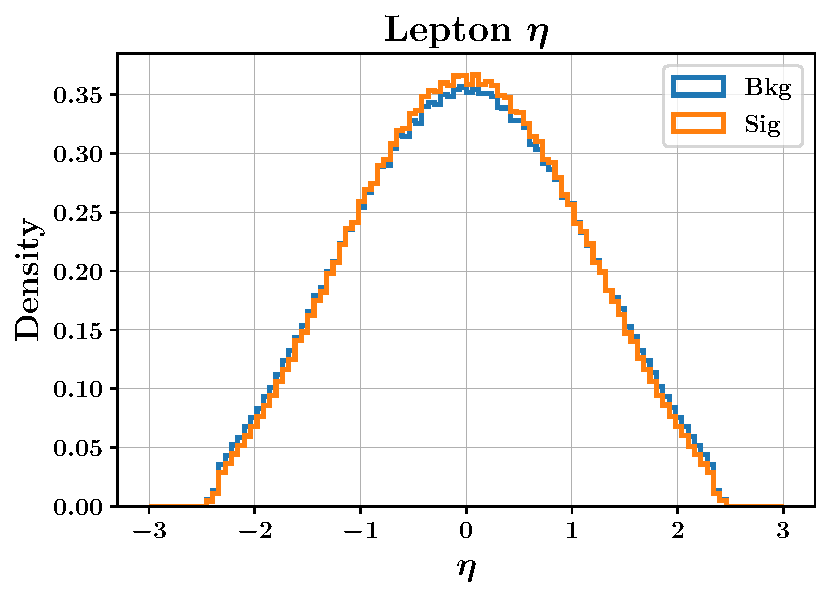
\includegraphics[width=\textwidth]{images/theory/lowlevel/l_eta.pdf}
%             \label{fig:appendix_low_features_leptonic_l_eta}
%         }
%     \end{minipage}%
%     \begin{minipage}[c]{0.333\linewidth}
%         \vspace{0pt}
%         \centering
%         \subfloat[Lepton \( \phi \)]{
%             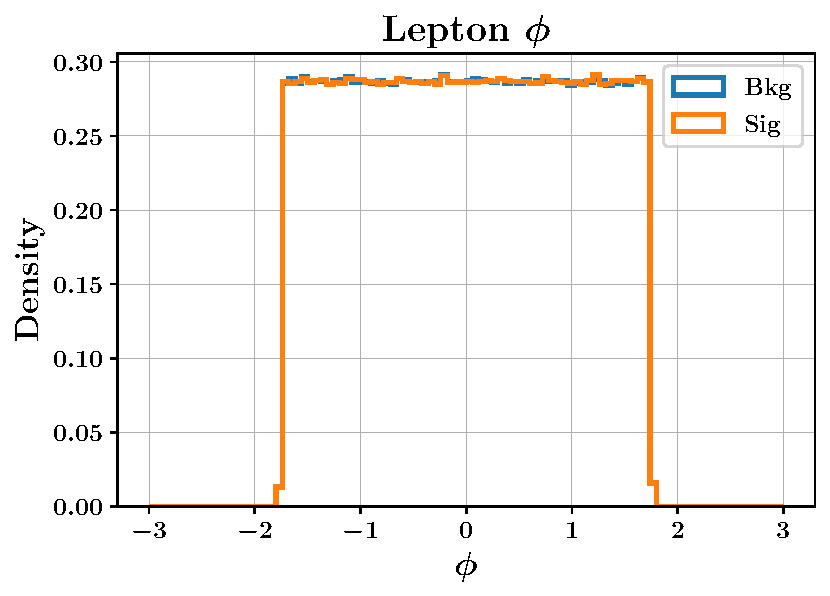
\includegraphics[width=\textwidth]{images/theory/lowlevel/l_phi.pdf}
%             \label{fig:appendix_low_features_leptonic_l_phi}
%         }
%     \end{minipage}%
    
%     \begin{minipage}[c]{0.165\linewidth}
%         \vspace{0pt}%
%         \hfill%
%     \end{minipage}%
%     \begin{minipage}[c]{0.333\linewidth}
%         \vspace{0pt}
%         \centering
%         \subfloat[Missing energy \( \slashed{E} \)]{
%             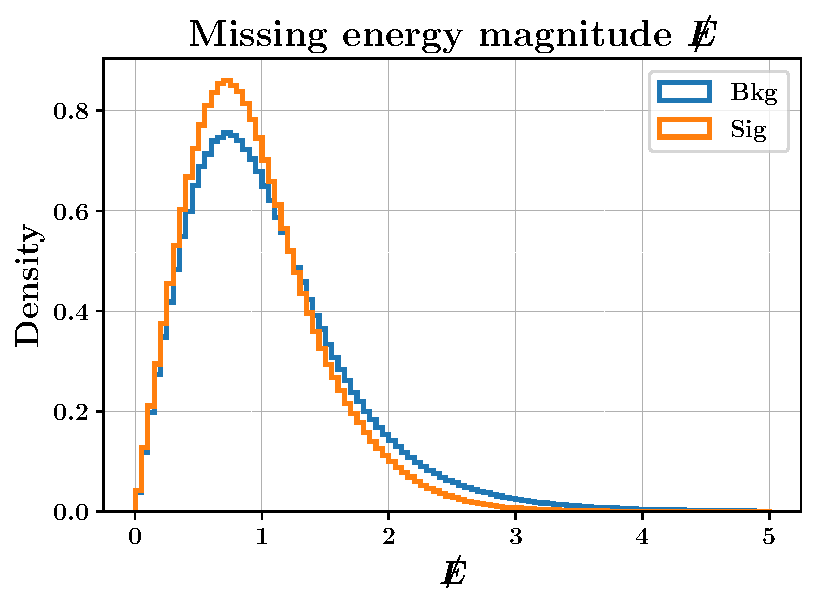
\includegraphics[width=\textwidth]{images/theory/lowlevel/miss_E_mag.pdf}
%             \label{fig:appendix_low_features_leptonic_miss_E_mag}
%         }
%     \end{minipage}%
%     \begin{minipage}[c]{0.333\linewidth}
%         \vspace{0pt}
%         \centering
%         \subfloat[Missing energy \( \slashed{\phi} \)]{
%             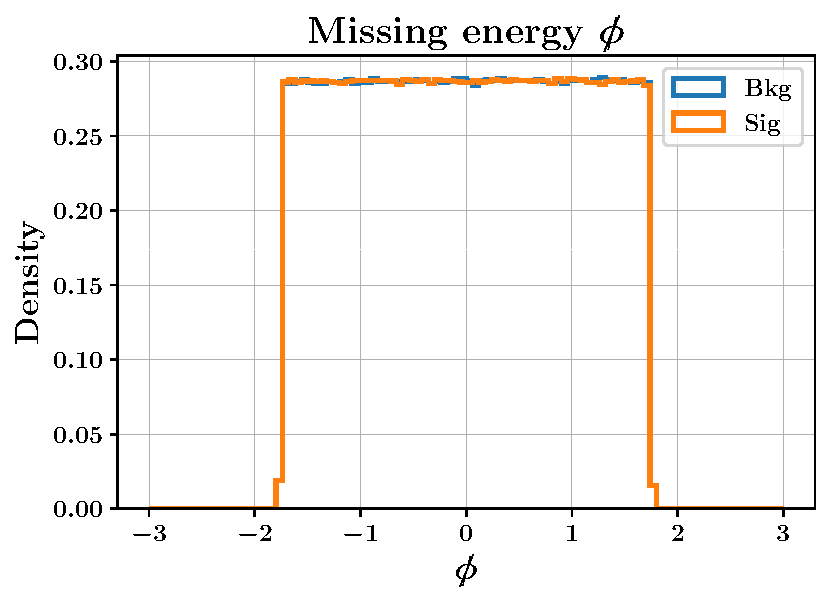
\includegraphics[width=\textwidth]{images/theory/lowlevel/miss_E_phi.pdf}
%             \label{fig:appendix_low_features_leptonic_miss_E_phi}
%         }
%     \end{minipage}%
%     \begin{minipage}[c]{0.165\linewidth}
%         \vspace{0pt}%
%         \hfill%
%     \end{minipage}%
%     \caption{Distributions of low-level features for the leptonic part for both background (blue line) and signal (orange line) events. Note that the dataset is given with a sort of normalisation already applied, so the features are expressed as pure numbers without the physical unit of measure.}
%     \label{fig:appendix_low_features_leptonic}
% \end{figure*}



% \clearpage


\begin{figure*}[!h]
    \begin{minipage}[c]{0.20\linewidth}
        \vspace{0pt}
        \centering
        \subfloat[Lepton \( p_{\text{T}} \)]{
            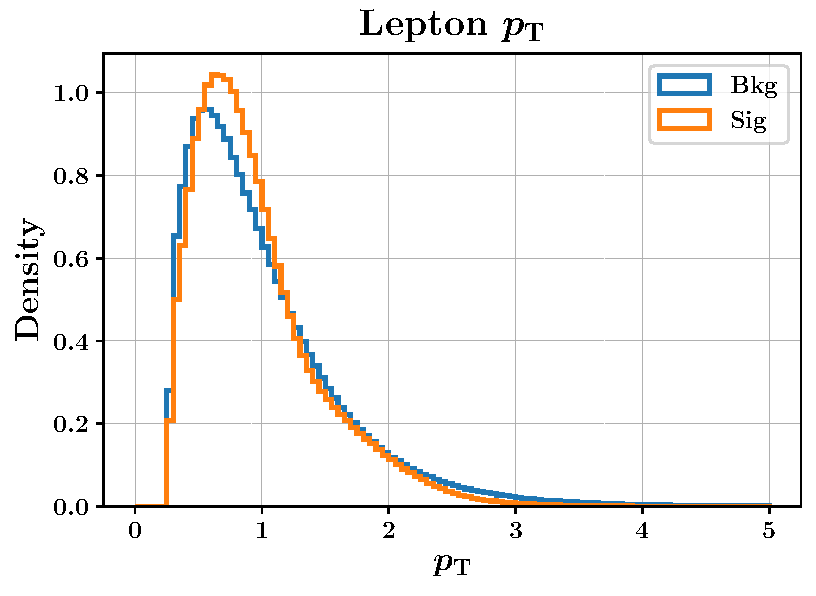
\includegraphics[width=\textwidth]{images/theory/lowlevel/l_pt.pdf}
            \label{fig:appendix_low_features_leptonic_l_pt}
        }
    \end{minipage}%
    \begin{minipage}[c]{0.20\linewidth}
        \vspace{0pt}
        \centering
        \subfloat[Lepton \( \eta \)]{
            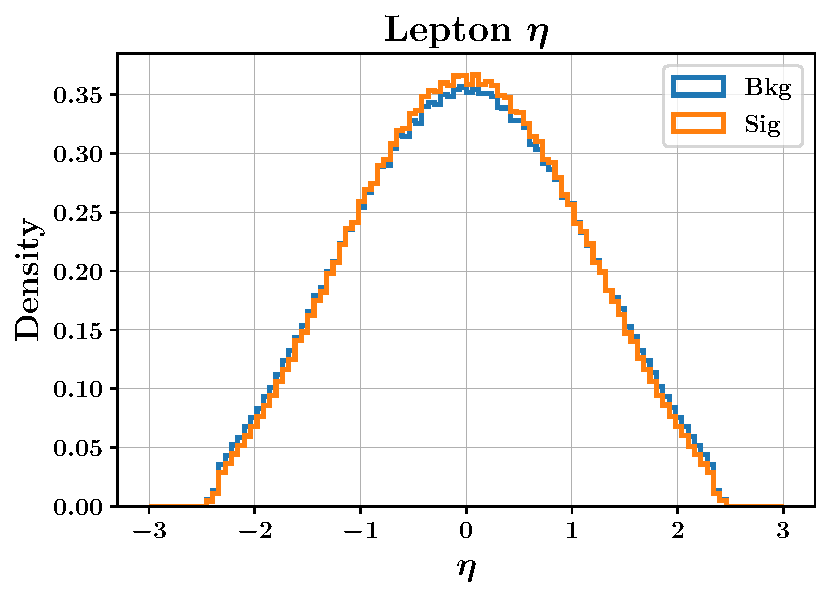
\includegraphics[width=\textwidth]{images/theory/lowlevel/l_eta.pdf}
            \label{fig:appendix_low_features_leptonic_l_eta}
        }
    \end{minipage}%
    \begin{minipage}[c]{0.20\linewidth}
        \vspace{0pt}
        \centering
        \subfloat[Lepton \( \phi \)]{
            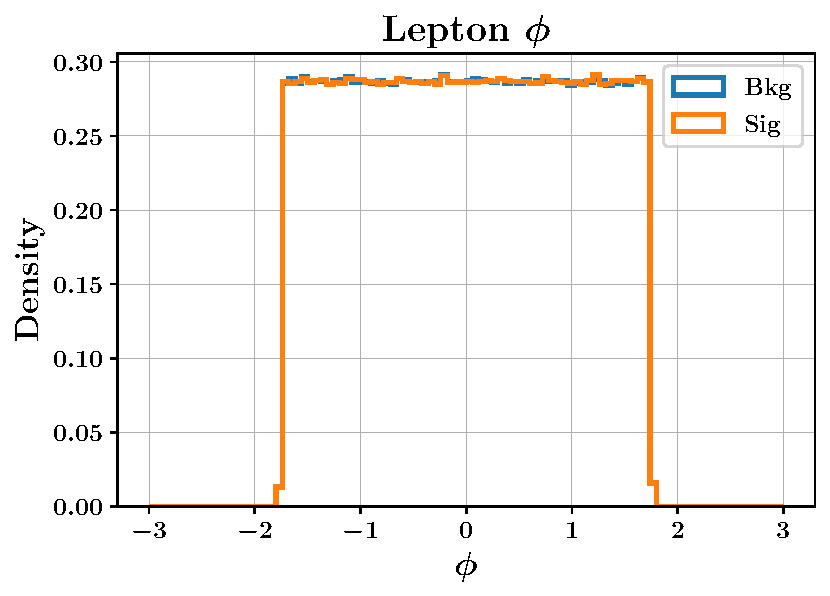
\includegraphics[width=\textwidth]{images/theory/lowlevel/l_phi.pdf}
            \label{fig:appendix_low_features_leptonic_l_phi}
        }
    \end{minipage}%
    \begin{minipage}[c]{0.20\linewidth}
        \vspace{0pt}
        \centering
        \subfloat[Missing energy \( \slashed{E} \)]{
            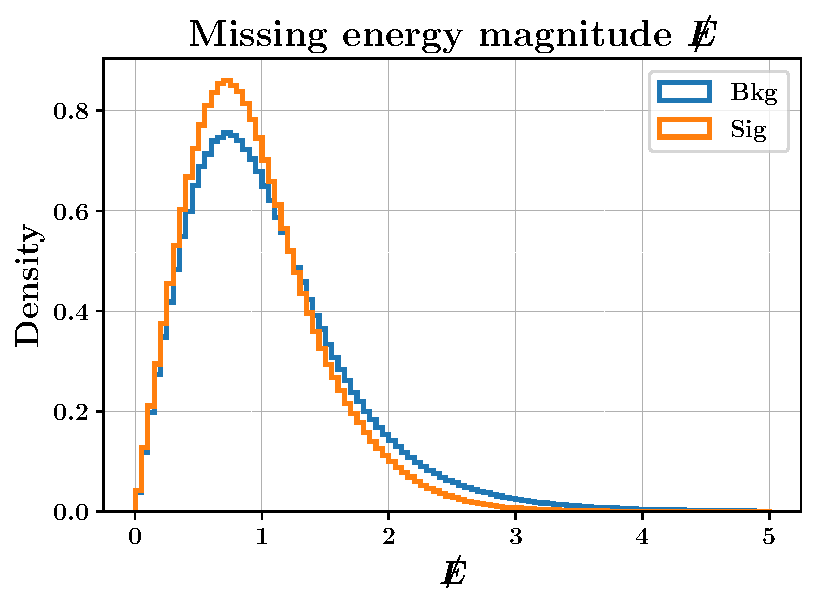
\includegraphics[width=\textwidth]{images/theory/lowlevel/miss_E_mag.pdf}
            \label{fig:appendix_low_features_leptonic_miss_E_mag}
        }
    \end{minipage}%
    \begin{minipage}[c]{0.20\linewidth}
        \vspace{0pt}
        \centering
        \subfloat[Missing energy \( \slashed{\phi} \)]{
            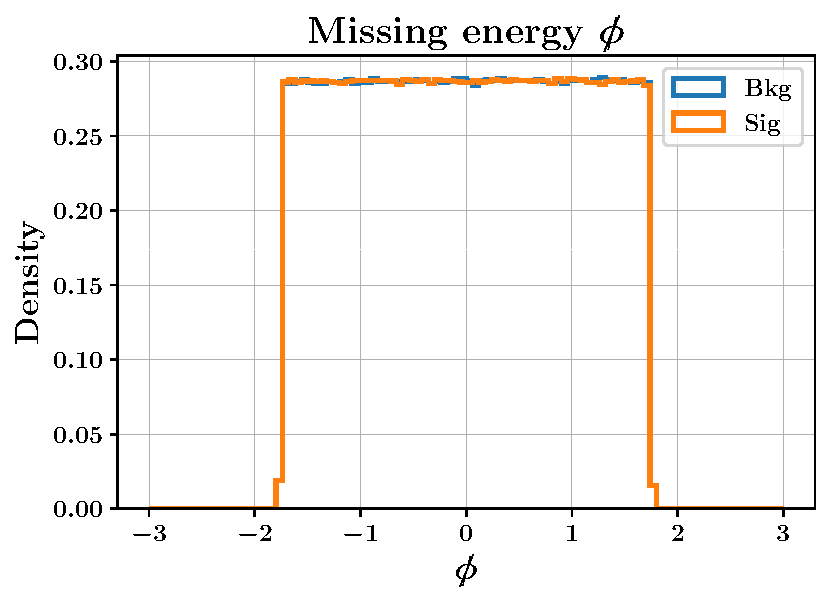
\includegraphics[width=\textwidth]{images/theory/lowlevel/miss_E_phi.pdf}
            \label{fig:appendix_low_features_leptonic_miss_E_phi}
        }
    \end{minipage}%
    \caption{Distributions of low-level features of leptonic part for background (blue) and signal (orange) events. The physical units of measure are omitted due to the fact that the dataset is not available in non-standardised form.}
    \label{fig:appendix_low_features_leptonic}
\end{figure*}

\vspace{-5mm}
\begin{figure*}[!h]
    \begin{minipage}[c]{0.25\linewidth}
        \vspace{0pt}
        \centering
        \subfloat[Jet 1: \( p_{\text{T}} \)]{
            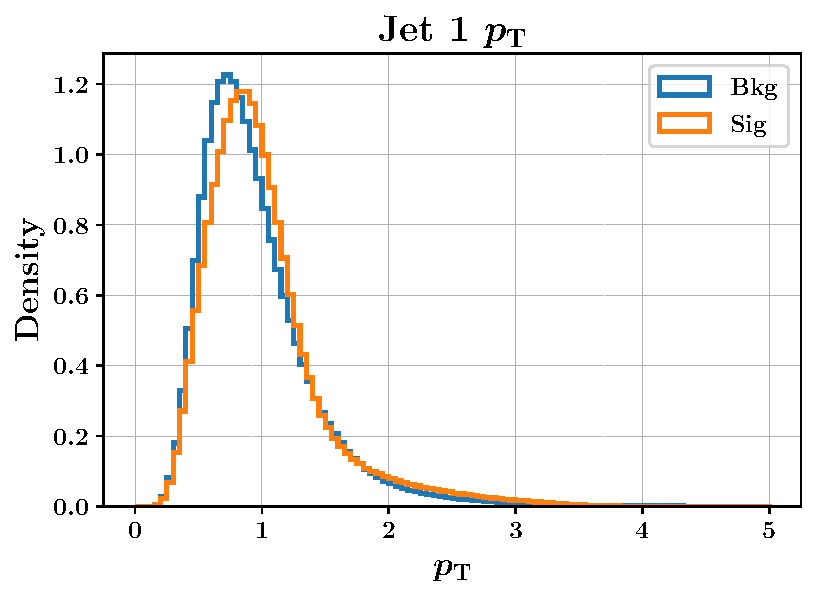
\includegraphics[width=\textwidth]{images/theory/lowlevel/j1_pt.pdf}
            \label{fig:appendix_low_features_hadronic_j1_pt}
        }
    \end{minipage}%
    \begin{minipage}[c]{0.25\linewidth}
        \vspace{0pt}
        \centering
        \subfloat[Jet 1: \( \eta \)]{
            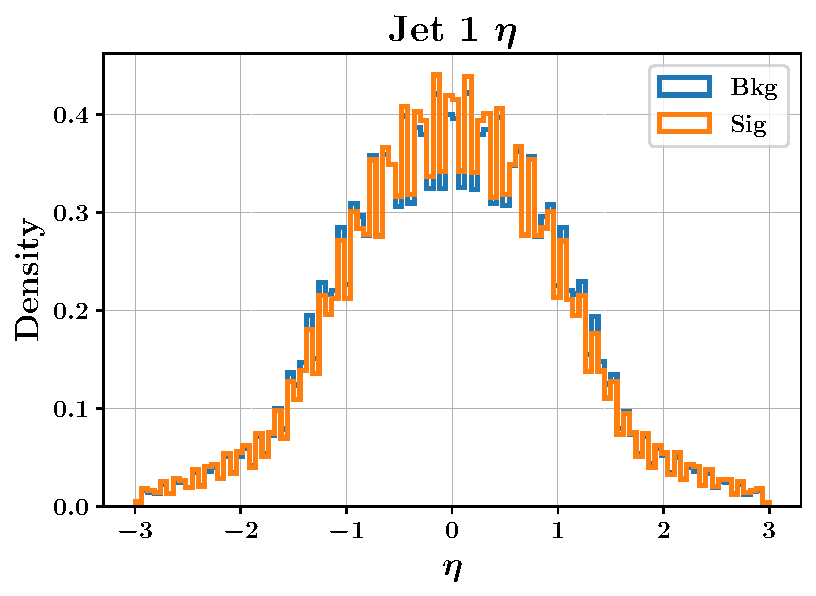
\includegraphics[width=\textwidth]{images/theory/lowlevel/j1_eta.pdf}
            \label{fig:appendix_low_features_hadronic_j1_eta}
        }
    \end{minipage}%
    \begin{minipage}[c]{0.25\linewidth}
        \vspace{0pt}
        \centering
        \subfloat[Jet 1: \( \phi \)]{
            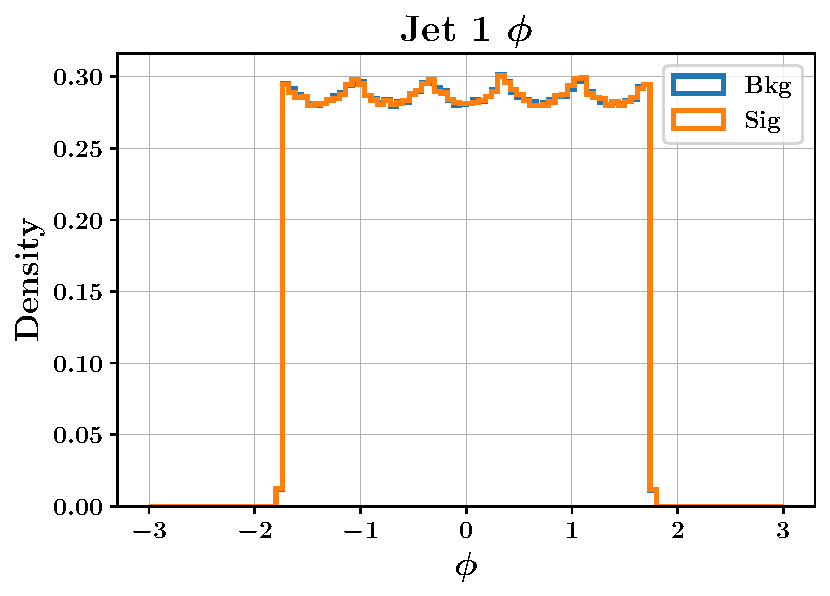
\includegraphics[width=\textwidth]{images/theory/lowlevel/j1_phi.pdf}
            \label{fig:appendix_low_features_hadronic_j1_phi}
        }
    \end{minipage}%
    \begin{minipage}[c]{0.25\linewidth}
        \vspace{0pt}
        \centering
        \subfloat[Jet 1: \( b \)-tag]{
            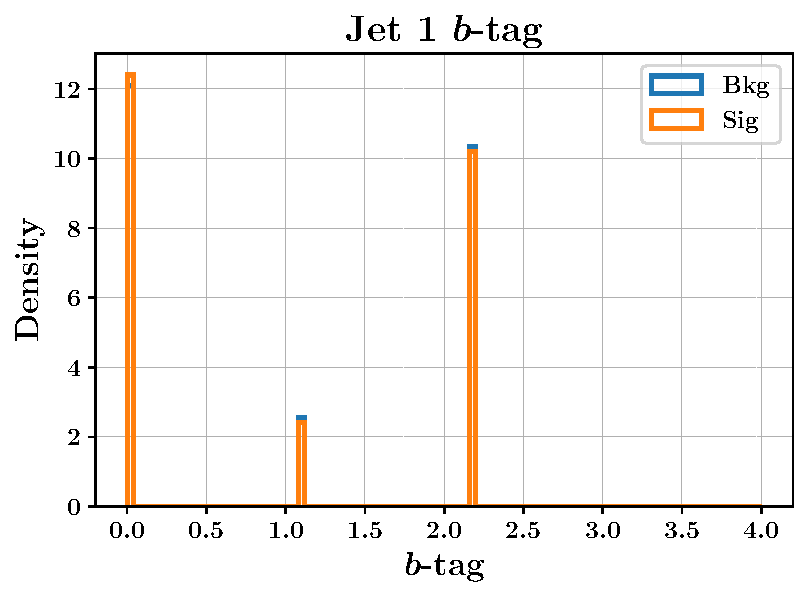
\includegraphics[width=\textwidth]{images/theory/lowlevel/j1_btag.pdf}
            \label{fig:appendix_low_features_hadronic_j1_btag}
        }
    \end{minipage}%
    
    \begin{minipage}[c]{0.25\linewidth}
        \vspace{0pt}
        \centering
        \subfloat[Jet 2: \( p_{\text{T}} \)]{
            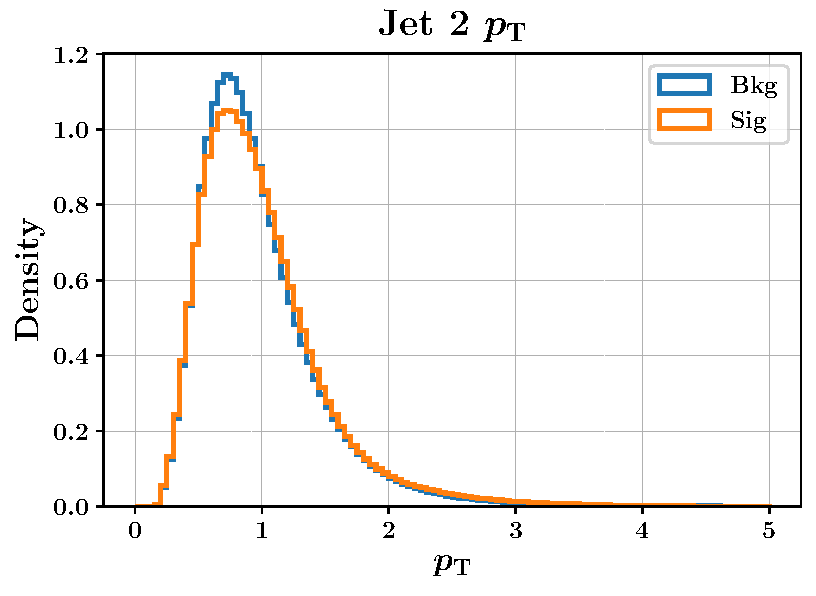
\includegraphics[width=\textwidth]{images/theory/lowlevel/j2_pt.pdf}
            \label{fig:appendix_low_features_hadronic_j2_pt}
        }
    \end{minipage}%
    \begin{minipage}[c]{0.25\linewidth}
        \vspace{0pt}
        \centering
        \subfloat[Jet 2: \( \eta \)]{
            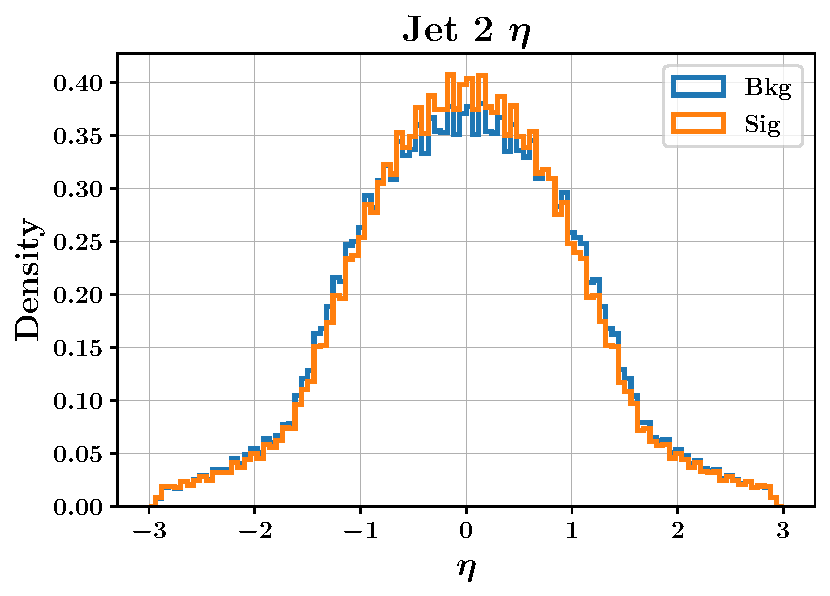
\includegraphics[width=\textwidth]{images/theory/lowlevel/j2_eta.pdf}
            \label{fig:appendix_low_features_hadronic_j2_eta}
        }
    \end{minipage}%
    \begin{minipage}[c]{0.25\linewidth}
        \vspace{0pt}
        \centering
        \subfloat[Jet 2: \( \phi \)]{
            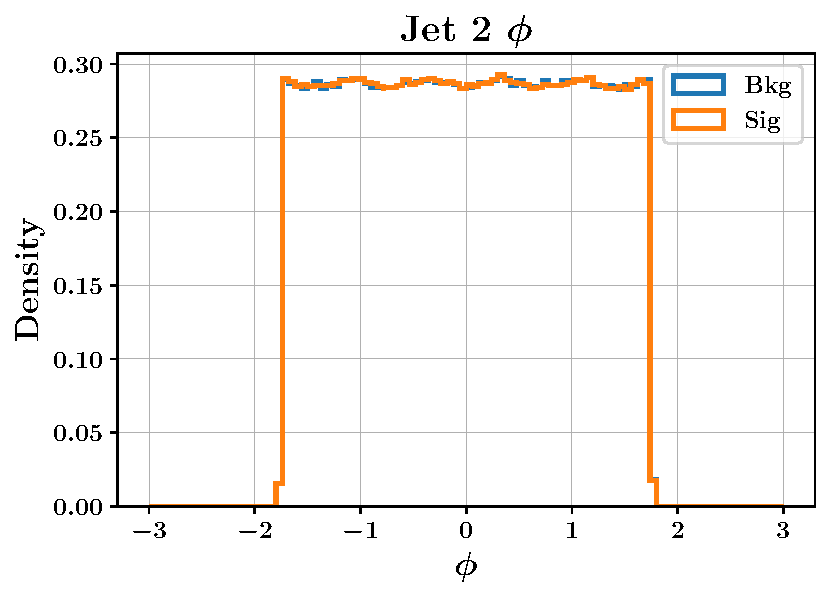
\includegraphics[width=\textwidth]{images/theory/lowlevel/j2_phi.pdf}
            \label{fig:appendix_low_features_hadronic_j2_phi}
        }
    \end{minipage}%
    \begin{minipage}[c]{0.25\linewidth}
        \vspace{0pt}
        \centering
        \subfloat[Jet 2: \( b \)-tag]{
            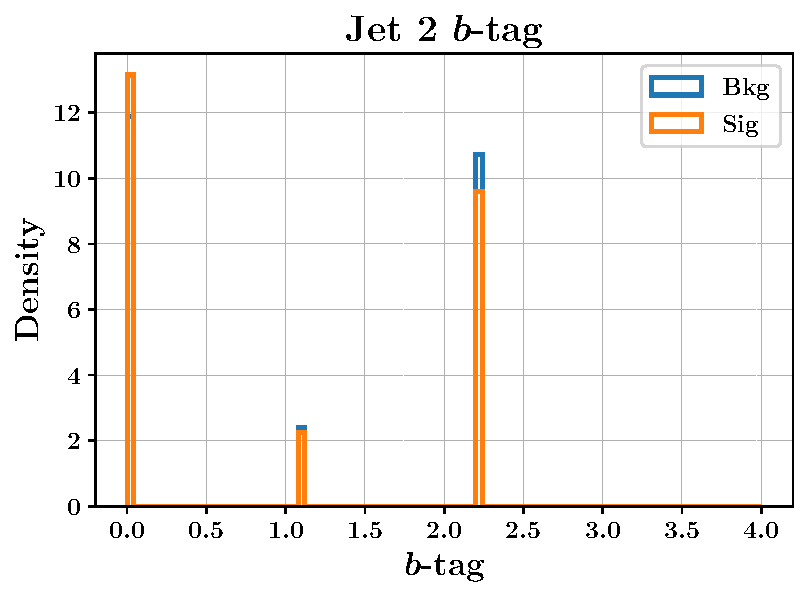
\includegraphics[width=\textwidth]{images/theory/lowlevel/j2_btag.pdf}
            \label{fig:appendix_low_features_hadronic_j2_btag}
        }
    \end{minipage}%
    
    \begin{minipage}[c]{0.25\linewidth}
        \vspace{0pt}
        \centering
        \subfloat[Jet 3: \( p_{\text{T}} \)]{
            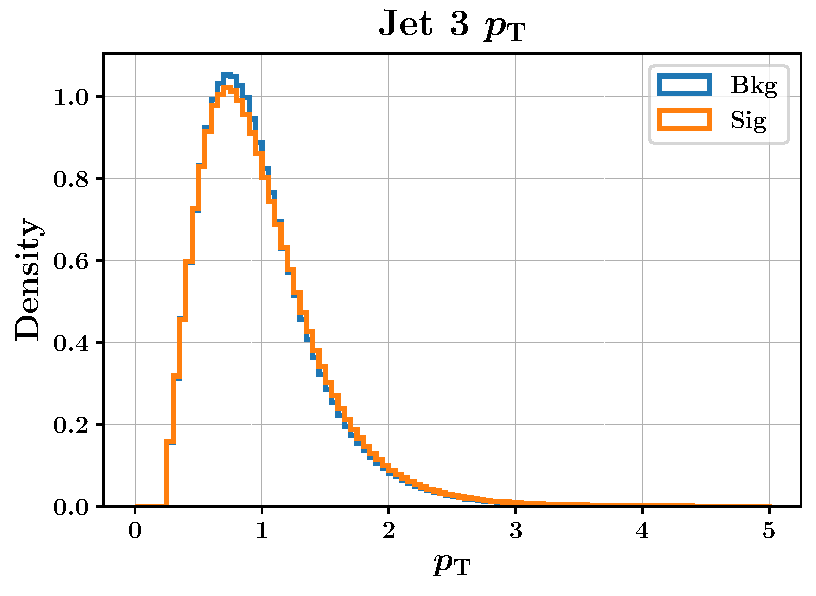
\includegraphics[width=\textwidth]{images/theory/lowlevel/j3_pt.pdf}
            \label{fig:appendix_low_features_hadronic_j3_pt}
        }
    \end{minipage}%
    \begin{minipage}[c]{0.25\linewidth}
        \vspace{0pt}
        \centering
        \subfloat[Jet 3: \( \eta \)]{
            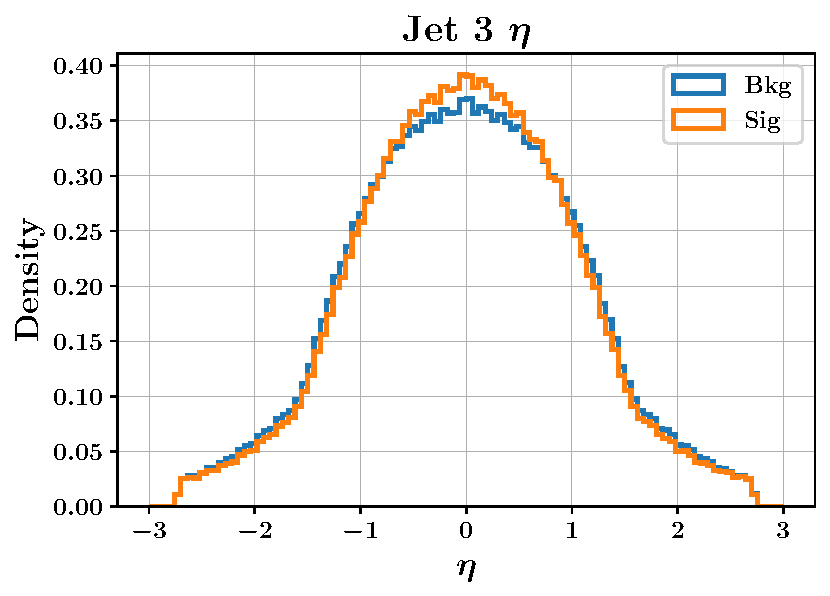
\includegraphics[width=\textwidth]{images/theory/lowlevel/j3_eta.pdf}
            \label{fig:appendix_low_features_hadronic_j3_eta}
        }
    \end{minipage}%
    \begin{minipage}[c]{0.25\linewidth}
        \vspace{0pt}
        \centering
        \subfloat[Jet 3: \( \phi \)]{
            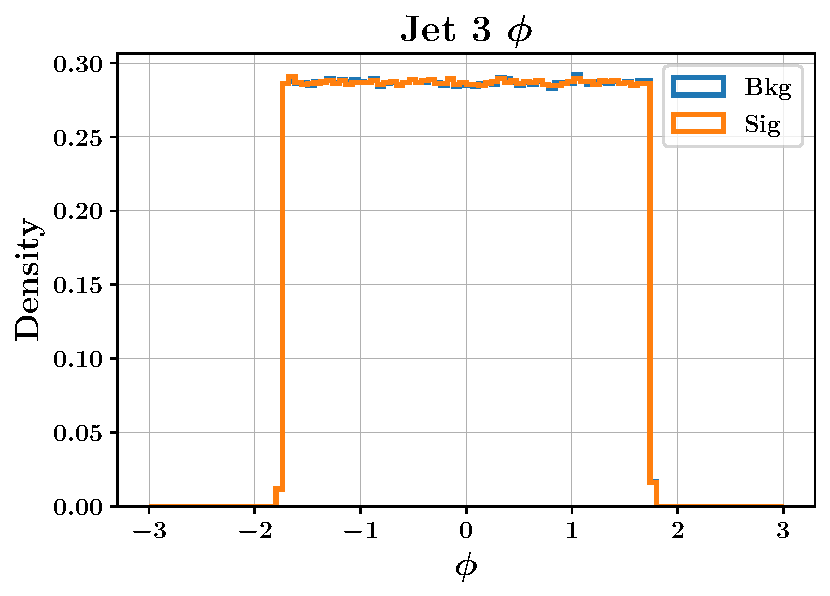
\includegraphics[width=\textwidth]{images/theory/lowlevel/j3_phi.pdf}
            \label{fig:appendix_low_features_hadronic_j3_phi}
        }
    \end{minipage}%
    \begin{minipage}[c]{0.25\linewidth}
        \vspace{0pt}
        \centering
        \subfloat[Jet 3: \( b \)-tag]{
            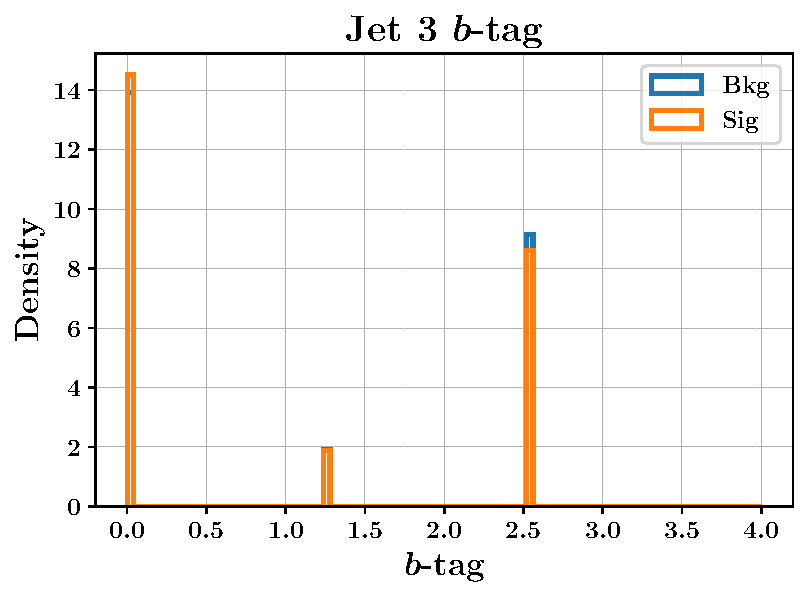
\includegraphics[width=\textwidth]{images/theory/lowlevel/j3_btag.pdf}
            \label{fig:appendix_low_features_hadronic_j3_btag}
        }
    \end{minipage}%
    
    \begin{minipage}[c]{0.25\linewidth}
        \vspace{0pt}
        \centering
        \subfloat[Jet 4: \( p_{\text{T}} \)]{
            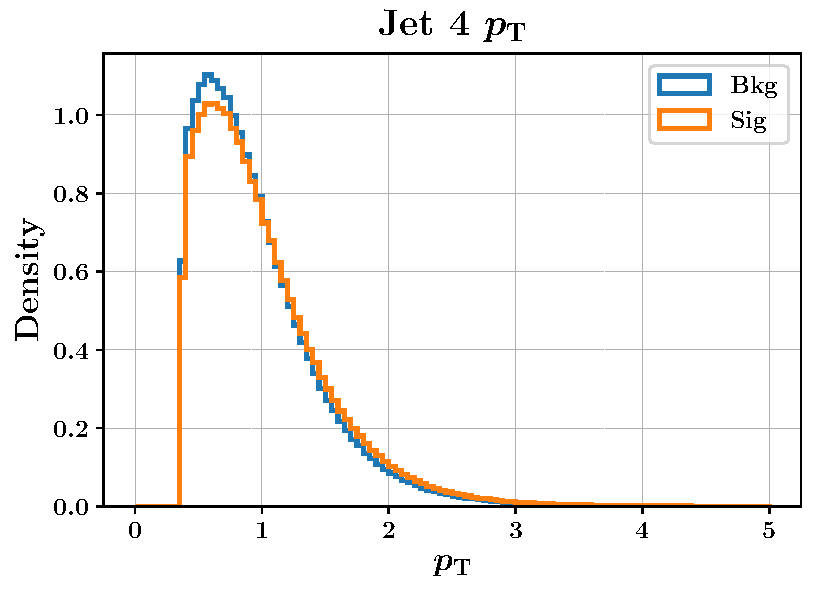
\includegraphics[width=\textwidth]{images/theory/lowlevel/j4_pt.pdf}
            \label{fig:appendix_low_features_hadronic_j4_pt}
        }
    \end{minipage}%
    \begin{minipage}[c]{0.25\linewidth}
        \vspace{0pt}
        \centering
        \subfloat[Jet 4: \( \eta \)]{
            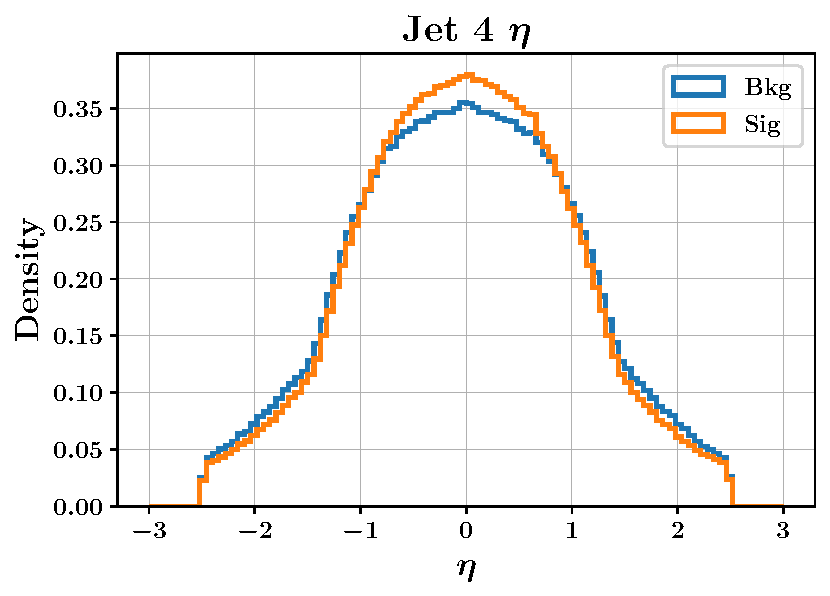
\includegraphics[width=\textwidth]{images/theory/lowlevel/j4_eta.pdf}
            \label{fig:appendix_low_features_hadronic_j4_eta}
        }
    \end{minipage}%
    \begin{minipage}[c]{0.25\linewidth}
        \vspace{0pt}
        \centering
        \subfloat[Jet 4: \( \phi \)]{
            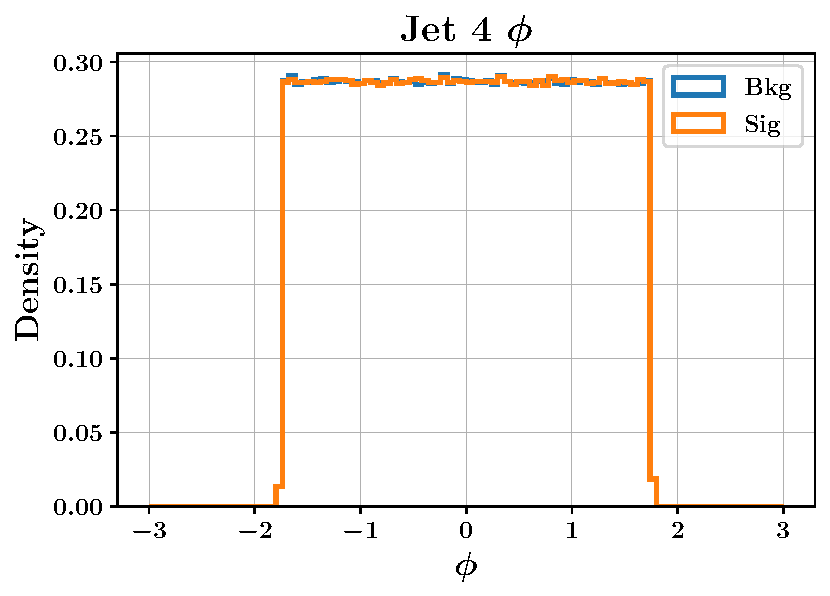
\includegraphics[width=\textwidth]{images/theory/lowlevel/j4_phi.pdf}
            \label{fig:appendix_low_features_hadronic_j4_phi}
        }
    \end{minipage}%
    \begin{minipage}[c]{0.25\linewidth}
        \vspace{0pt}
        \centering
        \subfloat[Jet 4: \( b \)-tag]{
            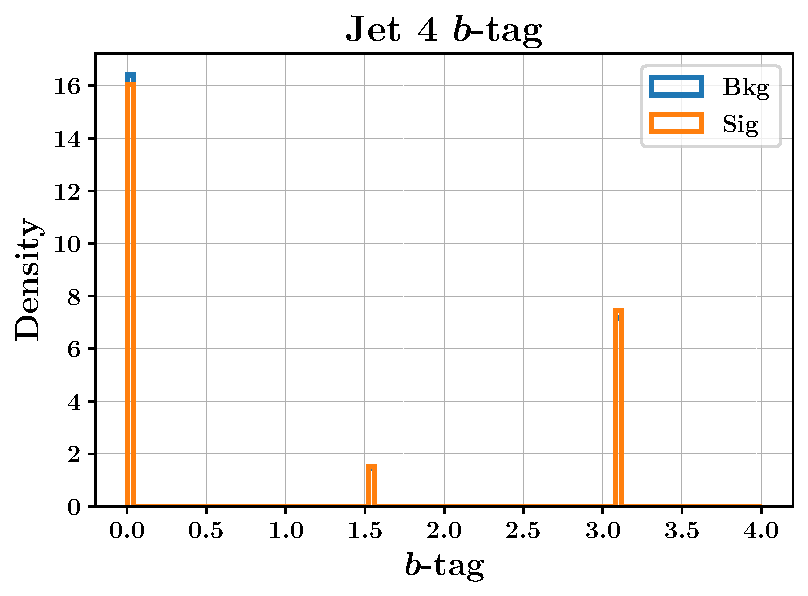
\includegraphics[width=\textwidth]{images/theory/lowlevel/j4_btag.pdf}
            \label{fig:appendix_low_features_hadronic_j4_btag}
        }
    \end{minipage}%
    \caption{Distributions of low-level features of hadronic part for background (blue) and signal (orange) events. The physical units of measure are omitted due to the fact that the dataset is not available in non-standardised form.}
    \label{fig:appendix_low_features_hadronic}
\end{figure*}



\clearpage



\subsection{High-level features distributions}
\label{ssec:appendix_high_features}

\begin{figure*}[!h]
    \begin{minipage}[c]{0.333\linewidth}
        \vspace{0pt}
        \centering
        \subfloat[\( m_{jj} \)]{
            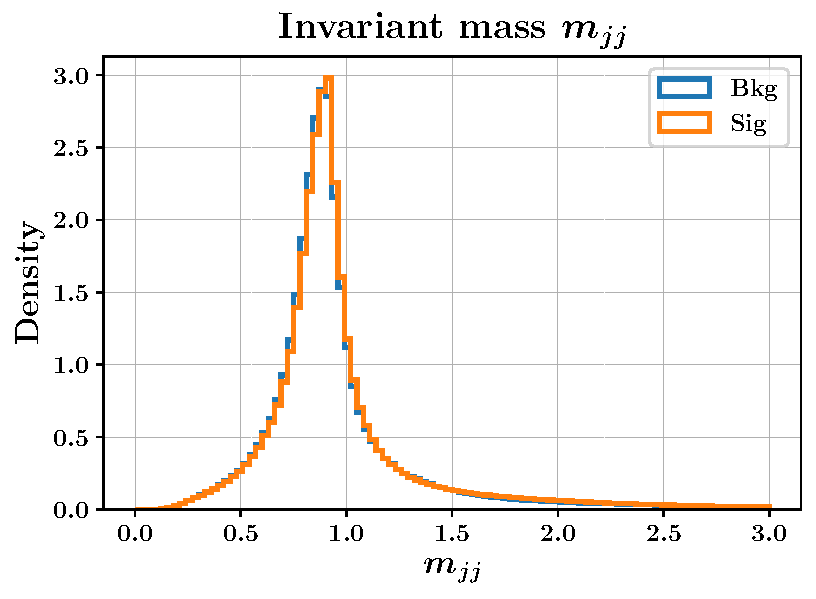
\includegraphics[width=\textwidth]{images/theory/highlevel/m_jj.pdf}
            \label{fig:appendix_high_features_m_jj}
        }
    \end{minipage}%
    \begin{minipage}[c]{0.333\linewidth}
        \vspace{0pt}
        \centering
        \subfloat[\( m_{jjj} \)]{
            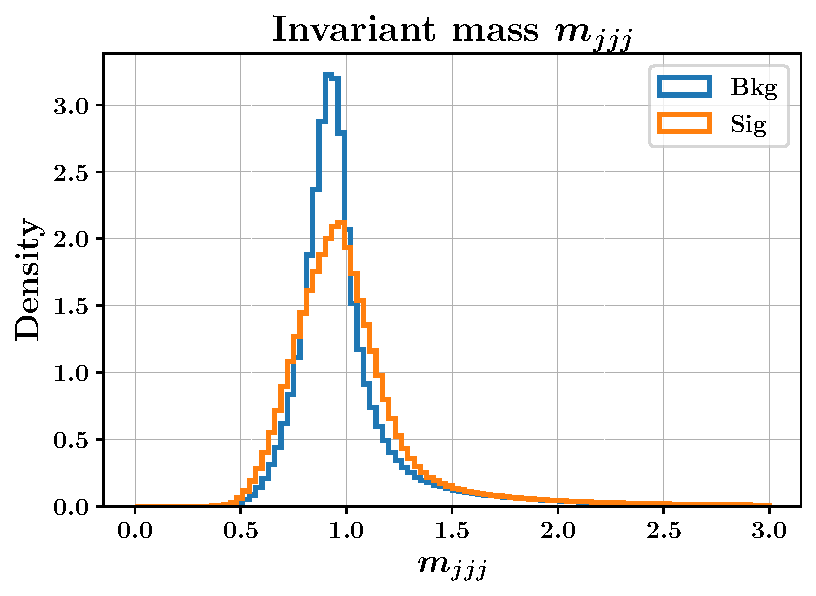
\includegraphics[width=\textwidth]{images/theory/highlevel/m_jjj.pdf}
            \label{fig:appendix_high_features_m_jjj}
        }
    \end{minipage}%
    \begin{minipage}[c]{0.333\linewidth}
        \vspace{0pt}
        \centering
        \subfloat[\( m_{\ell\nu} \)]{
            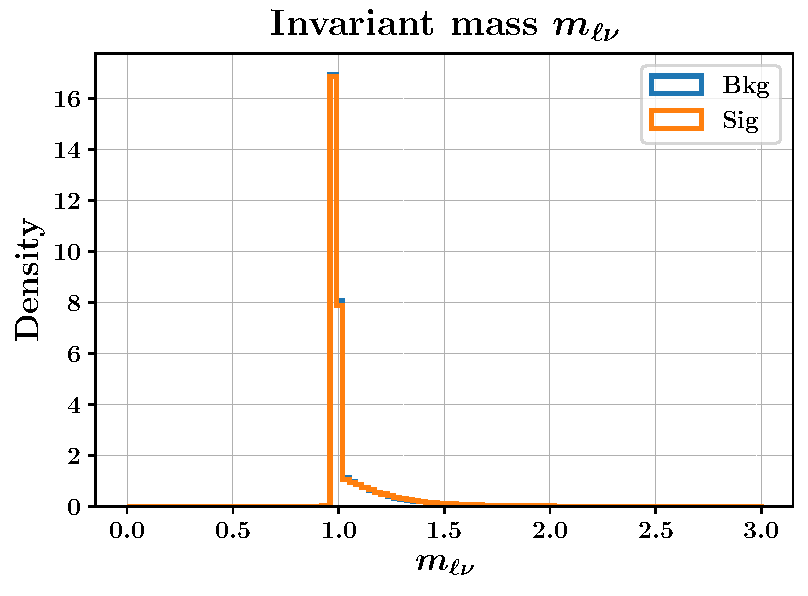
\includegraphics[width=\textwidth]{images/theory/highlevel/m_lv.pdf}
            \label{fig:appendix_high_features_m_lv}
        }
    \end{minipage}%

    \begin{minipage}[c]{0.333\linewidth}
        \vspace{0pt}
        \centering
        \subfloat[\( m_{j\ell\nu} \)]{
            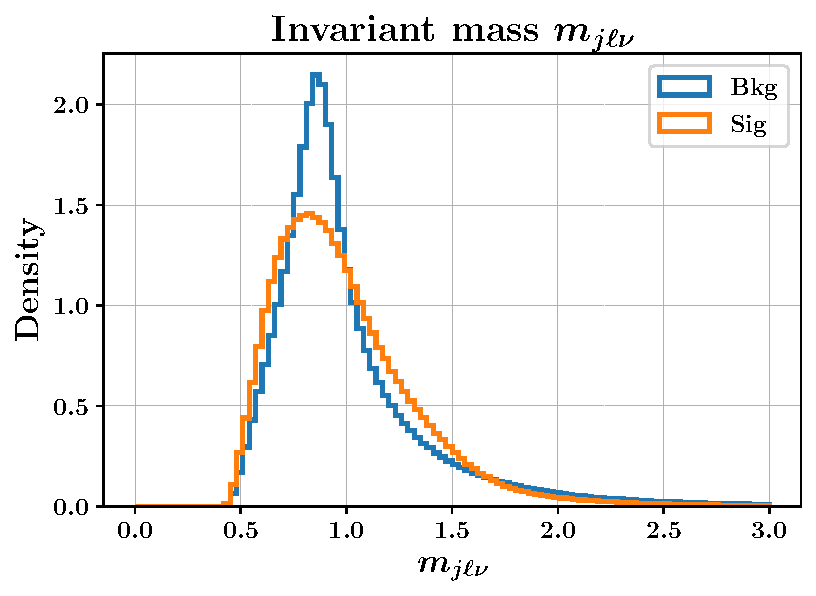
\includegraphics[width=\textwidth]{images/theory/highlevel/m_jlv.pdf}
            \label{fig:appendix_high_features_m_jlv}
        }
    \end{minipage}%
    \begin{minipage}[c]{0.333\linewidth}
        \vspace{0pt}
        \centering
        \subfloat[\( m_{bb} \)]{
            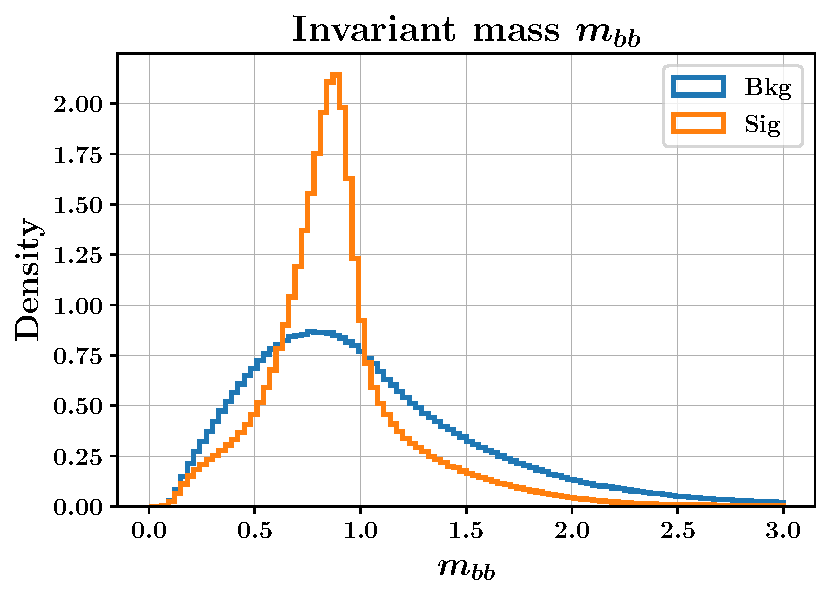
\includegraphics[width=\textwidth]{images/theory/highlevel/m_bb.pdf}
            \label{fig:appendix_high_features_m_bb}
        }
    \end{minipage}%
    \begin{minipage}[c]{0.333\linewidth}
        \vspace{0pt}
        \centering
        \subfloat[\( m_{Wbb} \)]{
            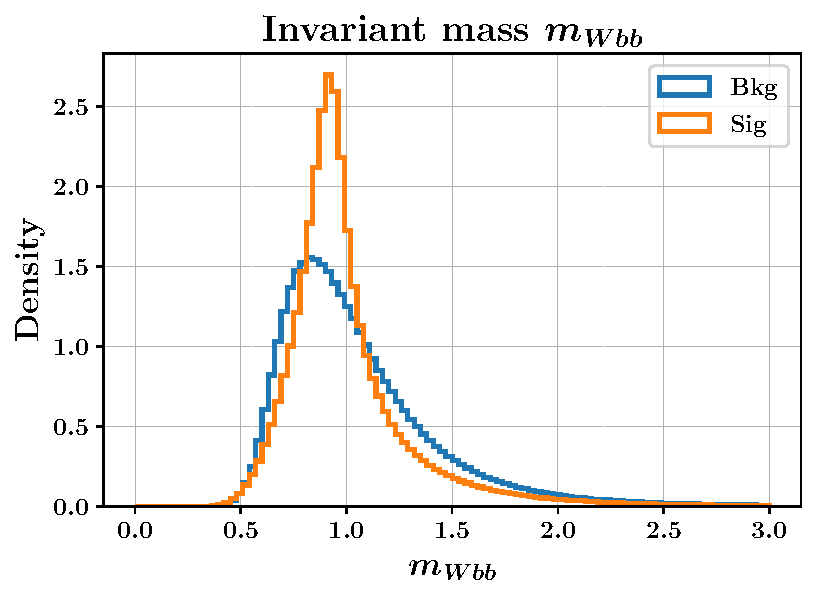
\includegraphics[width=\textwidth]{images/theory/highlevel/m_wbb.pdf}
            \label{fig:appendix_high_features_m_wbb}
        }
    \end{minipage}%
    
    \begin{minipage}[c]{0.333\linewidth}
        \vspace{0pt}
        \hfill
    \end{minipage}%
    \begin{minipage}[c]{0.333\linewidth}
        \vspace{0pt}
        \centering
        \subfloat[\( m_{WWbb} \)]{
            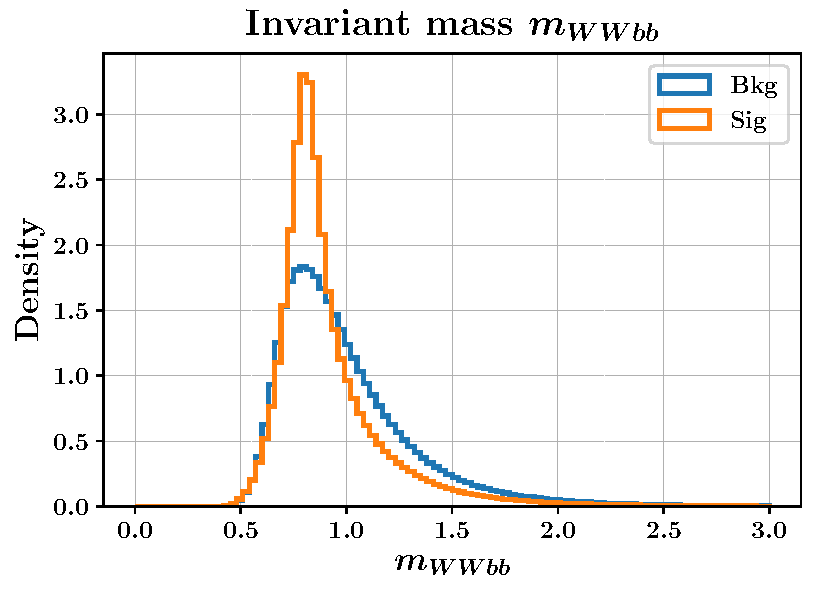
\includegraphics[width=\textwidth]{images/theory/highlevel/m_wwbb.pdf}
            \label{fig:appendix_high_features_m_wwbb}
        }
    \end{minipage}%
    \begin{minipage}[c]{0.333\linewidth}
        \vspace{0pt}
        \hfill
    \end{minipage}%
    \caption{Distributions of high-level features for background (blue) and signal (orange) events. The physical units of measure are omitted due to the fact that the dataset is not available in non-standardised form.}
    \label{fig:appendix_high_features}
\end{figure*}

\clearpage



\renewcommand{\lstlistingname}{\textbf{LST.}}
\renewcommand{\thelstlisting}{\textbf{\arabic{lstlisting}}}

\subsection{TTN constructors}
\label{ssec:appendix_constructors}

\begin{lstlisting}[
    style=mypython,
    frame=single,
    caption={Core implementation of a ``pure'' TTN structure constructor without the employment of advanced techniques, such as batch normalisation and regularisation.},
    captionpos=b,
    aboveskip=10pt,
    belowskip=10pt,
    label=lst:code_building_pure_structure
]
# first layer
tn_model.add(
    TTN_SingleNode(
        bond_dim      = bond_dim,
        n_contraction = n_contr
        use_bias      = True,
        activation    = activation,
        input_shape   = input_shape,
    )
)

# intermediate layers
for _ in range(n_layers-2):
    tn_model.add(
        TTN_SingleNode(
            bond_dim      = bond_dim,
            n_contraction = n_contr
            use_bias      = True,
            activation    = activation
        )
    )

# last layer
tn_model.add(
    TTN_SingleNode(
        bond_dim      = 1,
        n_contraction = n_contr
        use_bias      = True,
        activation    = 'sigmoid'
    )
)
\end{lstlisting}



\begin{lstlisting}[
    style=mypython,
    frame=single,
    caption={Core implementation of a more sophisticated TTN structure constructor with the employment of advanced techniques, such as batch normalisation and regularisation.},
    captionpos=b,
    aboveskip=10pt,
    belowskip=10pt,
    label=lst:code_building_advanced_structure
]
# first layer
tn_model.add(
    TTN_SingleNode(
        bond_dim           = bond_dim,
        n_contraction      = n_contr,
        use_bias           = use_bias,
        kernel_regularizer = kernel_regulariser
        input_shape        = input_shape,
    )
)
tn_model.add(
    BatchNormalization(
        epsilon  = 1e-06,
        momentum = 0.9,
        weights  = None
    )
)
if activation is not None:
    tn_model.add(Activation(activation))

# intermediate layers
for _ in range(n_layers-2):
    tn_model.add(
        TTN_SingleNode(
            bond_dim           = bond_dim,
            n_contraction      = n_contr,
            use_bias           = use_bias,
            kernel_regularizer = kernel_regulariser
        )
    )
    tn_model.add(
        BatchNormalization(
            epsilon  = 1e-06,
            momentum = 0.9,
            weights  = None
        )
    )
    if activation is not None:
        tn_model.add(Activation(activation))

# last layer with bond dimension 1
tn_model.add(
    TTN_SingleNode(
        bond_dim           = 1,
        use_bias           = True,
        n_contraction      = n_contr,
        input_shape        = input_shape,
        kernel_regularizer = kernel_regulariser
    )
)
tn_model.add(
    BatchNormalization(
        epsilon  = 1e-06,
        momentum = 0.9,
        weights  = None
    )
)
tn_model.add(Activation('sigmoid'))
\end{lstlisting}


\end{document}